%!TEX root = report.tex
\subsection{Experimental Results}

\subsubsection{Performance measure}
The performance of the localization can be quantified by the distance from the calculated target point to its real position (measured with a laser pointer). 
Both algorithms, fixed-height and free-height (see § \ref{sec:triangulation}), are applied. The errors in the x-y plane for fixed-height and free-height as well as the 3D error for free-height are considered. 

With the four available cameras there are several camera combinations that can be used for the calculation.
It was found that the error in the position of the robot is highly dependent on which cameras are used for triangulating the image points. 
Currently, the best camera combination is determined based on the error between the measured and actual position of the robot.
In later experimental setups, however, the real position of the robot will not be directly measured, so it is necessary to find another criterion for evaluating the camera combinations.
One option considered was to use the errors of the reprojection of the reference points, whose positions are already well-known.
The results of this approach, shown in Figure~\ref{fig:res0_err}, however, suggest that the correlation between the reference point error and the robot position error is not strong enough, so a different criterion needs to be found.
This task is beyond the scope of the present project so in the following section, all camera combinations are considered and the real position of the robot is used for measurement of performance.


\begin{figure}
    \centering
    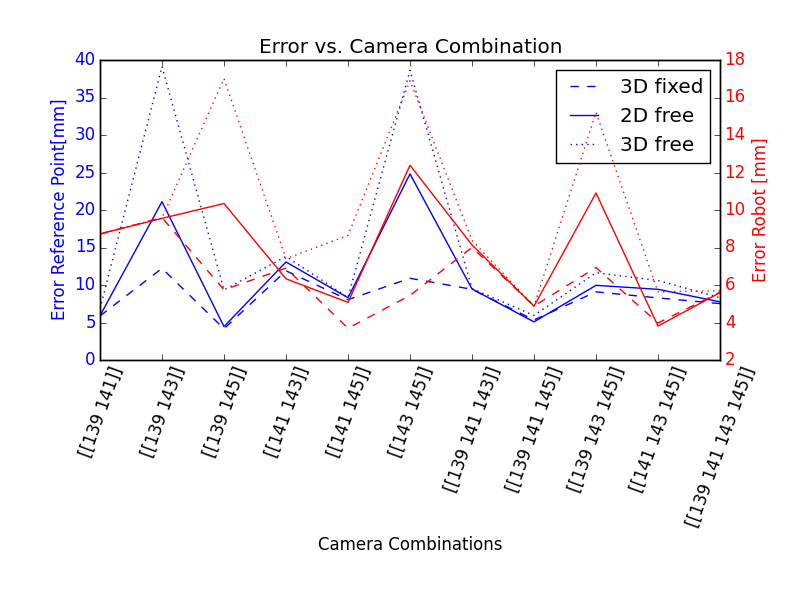
\includegraphics[width=.8\linewidth]{files/res0_combi_4.png}
    \caption{Experiment in Atrium: results of visual localization for various camera combinations.}
    \label{fig:res0_err}
\end{figure}

\subsubsection{Reference frames}
Two reference frames are used in the experiments. First, there is the point reference frame, in which the visual localization is done. 
In this frame, the x axis is defined to point from the first to the second reference point (\textit{ref basis} in Figure \ref{fig:res1_room} and \ref{fig:res2_room} ) and the z axis points out of the floor.
For visualization purposes, a margin in x and y direction is added to these points, so the origin is slightly offset from the basis line (see \textit{ref origin} in Figures \ref{fig:res1_room} and \ref{fig:res2_room}).

\subsubsection{Experiment in BC building hall (Atrium)}
The first experiments were done in the Atrium of the BC building, with 5 orange reference points for extrinsic calibration and a bottle as a target point instead of the robot.
This setup is characterized by a small height difference between the reference points (height 20 mm) and the target point (height 160 mm). 
The cameras are placed at a height of around 2 meters which leads to bottom-down views for all cameras (Figure \ref{fig:res0_img139} and \ref{fig:res0_img141}).
The resulting error of the bottle position is less than 18mm for all camera combinations and goes down to 5.8mm in 3D (cameras 139, 141, 145) or 4 mm in 2D with fixed height (cameras 139, 143) (see Figure~\ref{fig:res0_err}). 

\begin{figure}
    \centering
    \begin{subfigure}{0.49\linewidth}
        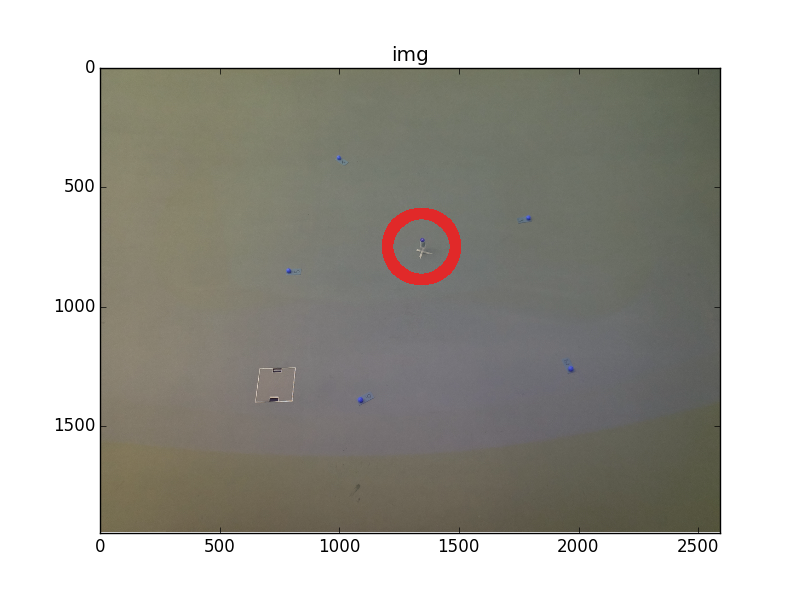
\includegraphics[width=\linewidth]{files/res0_img139.png}
        \caption{View from camera 139.}
        \label{fig:res0_img139}
    \end{subfigure}
    \begin{subfigure}{0.49\linewidth}
        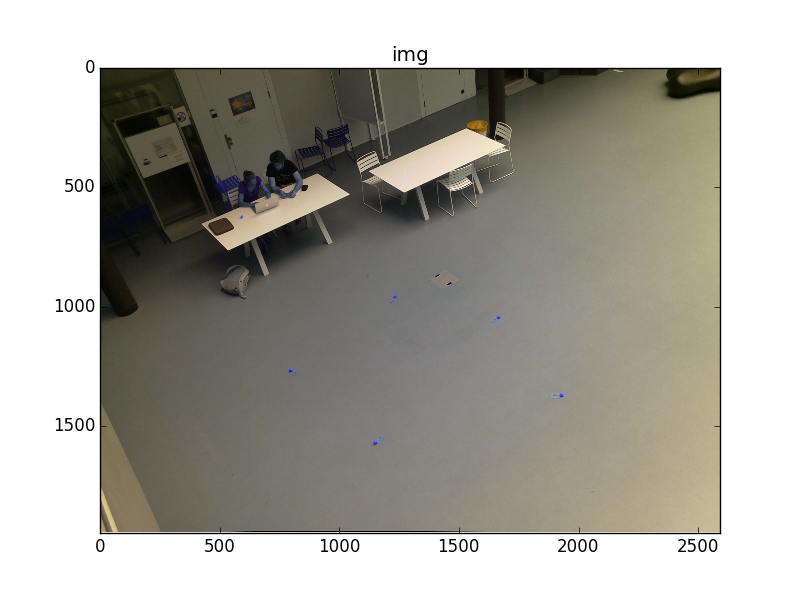
\includegraphics[width=\linewidth]{files/res0_img141.png}
        \caption{View from camera 141. }
        \label{fig:res0_img141}
    \end{subfigure}
    \caption{Experiment in Atrium: camera views with 5 blue reference points and the bottle as target point in view 139.}
    \label{fig:res0_views}
\end{figure}


\subsubsection{Experiment in BC329 with reference points}

A second experiment was performed in a more realistic setting in BC room 329, using 6 reference points for extrinsic calibration and the real robot as target point (see Figure \ref{fig:res1_img}). 
In addition to the visual localization, odometry was used to evaluate the position of the robot.
\begin{figure}
    \centering
    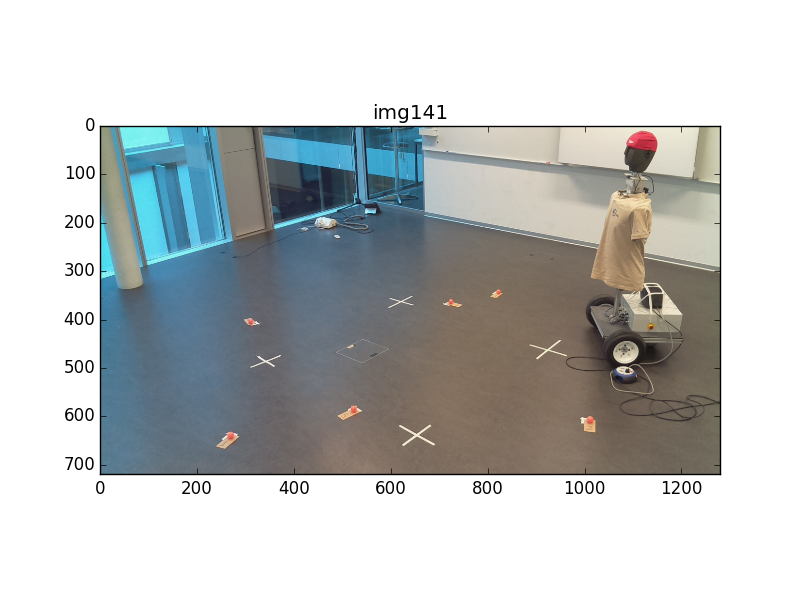
\includegraphics[width=.6\linewidth]{files/res1_img141.png}
    \caption{Experiment with reference points: view from camera 141.}
    \label{fig:res1_img}
\end{figure}
The performance of odometry was measured at 3 positions but because of technical issues, visual localization could only be performed at one position. 
The robot's real positions, measured positions within the room, and the placement of the cameras are illustrated in Figure \ref{fig:res1_room}.
The position calculated by visual localization is quite far from the real positions, which can be more clearly seen in Figure \ref{fig:res1_combi}. 

\begin{figure}
    \centering
    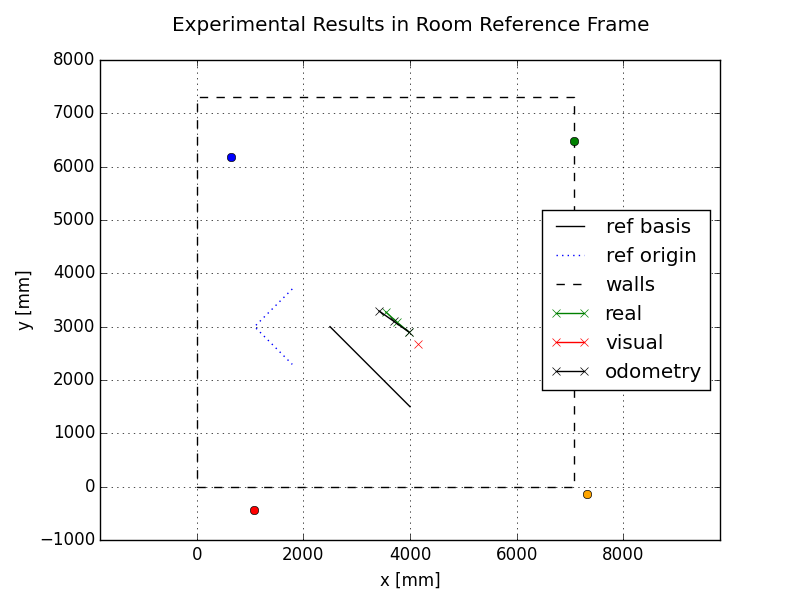
\includegraphics[width=.8\linewidth]{files/res1_room.png}
    \caption{Experiment with reference points: summary of results in room reference frame (Camera numbering: blue 139, red 141, green 143, orange 145).}
    \label{fig:res1_room}
\end{figure}

The best result is obtained with the camera combination (141,143); all other combinations give significantly higher error.
The resulting error (46 mm) from the best camera combination is still significantly higher than for the experiments in the Atrium, as the view is much less bottom-down, so small errors in height lead to large lateral errors.
A more closer look of the results reveils that the height of the robot is very badly determined when camera 145 is used. This is not a result of errors in the calculation of the position of the camera, which is as accurate as the others (Figure \ref{fig:res1_room}, orange point). 
It could be that its position relative to the robot is poorly chosen, as it is comparatively close to the robot head meaning that the calculated position is very sensitive to small changes in the robot position within the image (see Figure \ref{fig:res1_img145}).

\begin{figure}
    \centering
    \begin{subfigure}{0.49\linewidth}
        \centering
        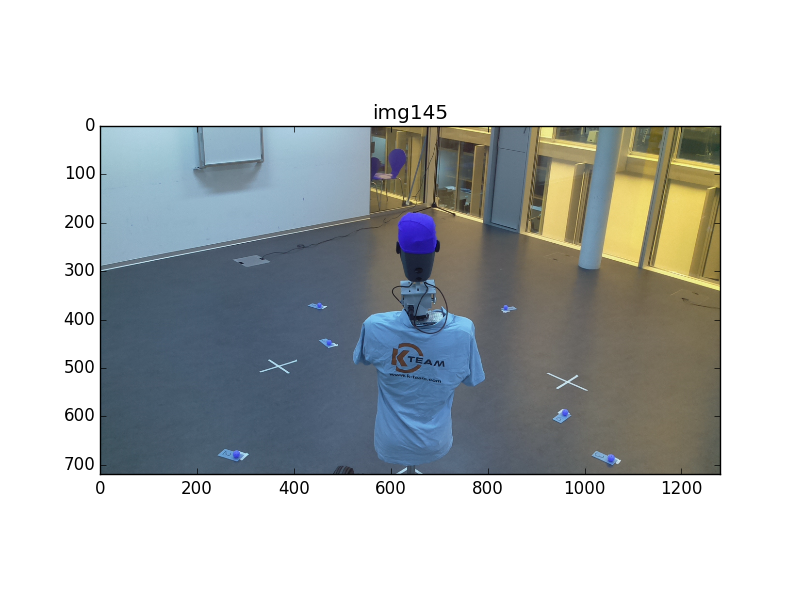
\includegraphics[width=\linewidth]{files/res1_img145.png}
        \caption{View from camera 145.}
        \label{fig:res1_img145}
    \end{subfigure}
    \begin{subfigure}{0.49\linewidth}
        \centering
        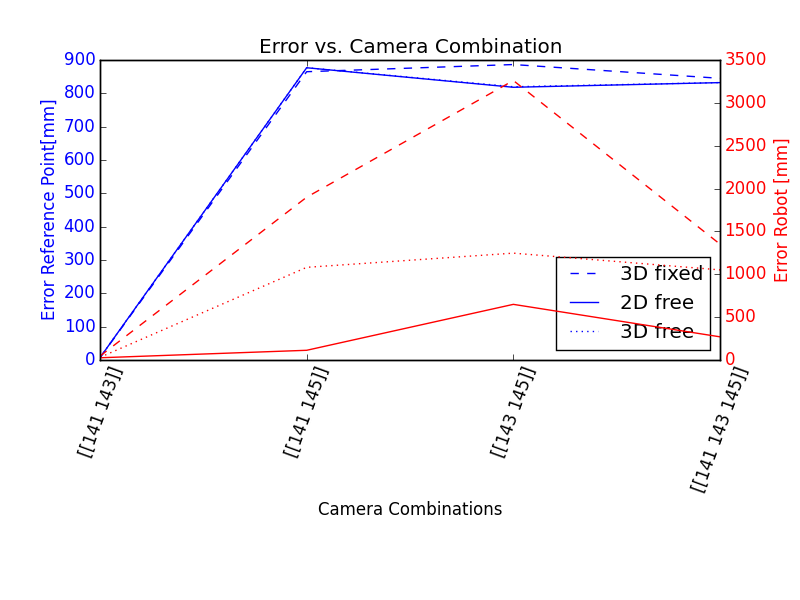
\includegraphics[width=\linewidth]{files/res1_combi_4.png}
        \caption{2D and 3D errors of 4th reference point and robot at the first position.}
        \label{fig:res1_combi}
    \end{subfigure}
    \caption{Experiment with reference points: view of badly positioning camera 145 and results of visual localization.}
    \label{fig:experiment1}
\end{figure}



\subsubsection{Experiment in BC329 with checkerboard}

A third experiment was performed in the same setting as above but using the checkerboard algorithm for extrinsic calibration instead of reference points (see Figures \ref{fig:res2_image_143} and  \ref{fig:res2_image_145}). 
The visual localization was performed at two locations and its results were significantly better than for the previous experiment. 

\begin{figure}
    \centering
    \begin{subfigure}{0.49\linewidth}
        \centering
        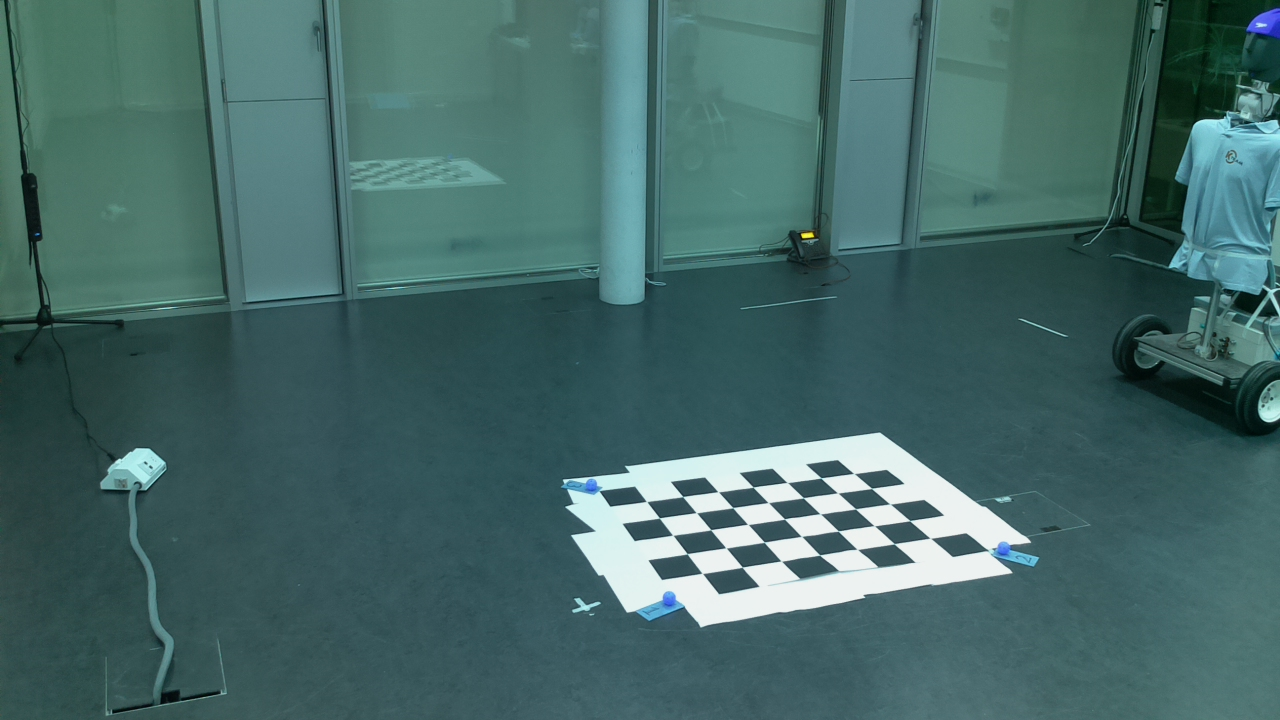
\includegraphics[width=\linewidth]{files/res2_image_143.png}
        \caption{View from camera 143.}
        \label{fig:res2_image_143}
    \end{subfigure}
    \begin{subfigure}{0.49\linewidth}
        \centering
        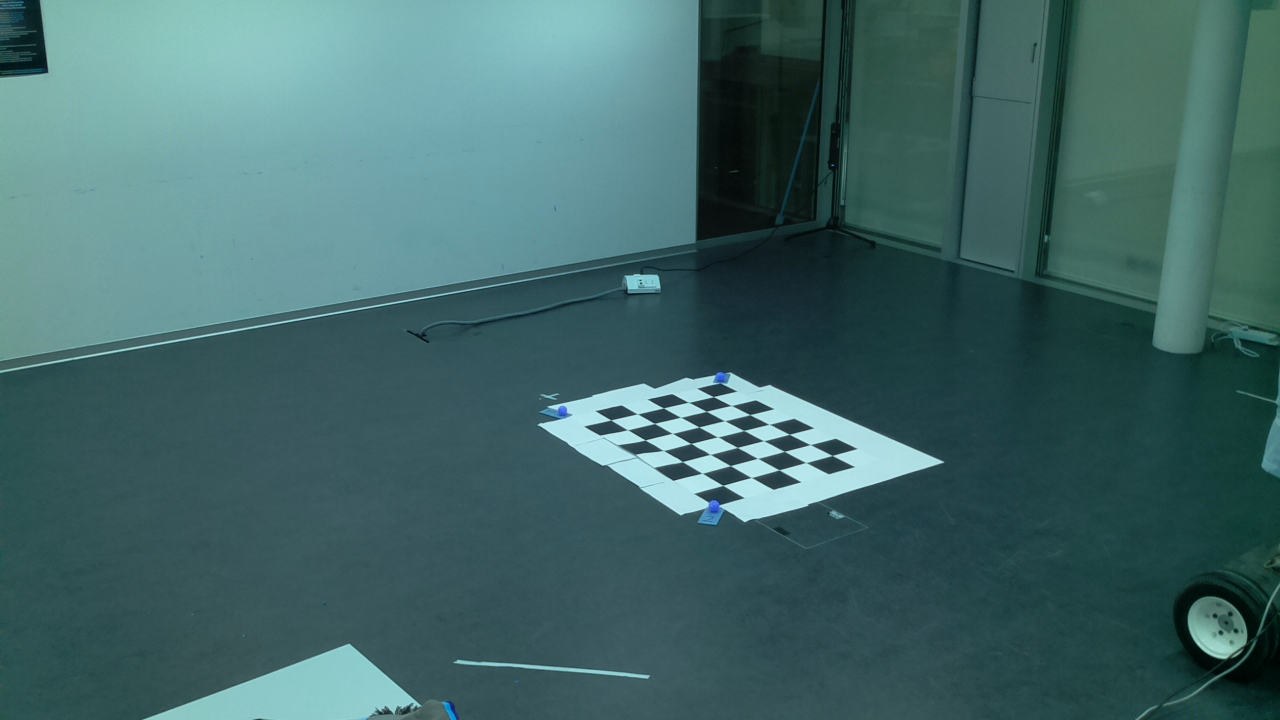
\includegraphics[width=\linewidth]{files/res2_image_145.png}
        \caption{View from camera 145.}
        \label{fig:res2_image_145}
    \end{subfigure}
    \caption{Experiment with checkerboard: camera views for extrinsic calibration.}
    \label{fig:experiment2}
\end{figure}

The robot position errors are shown in Figure \ref{fig:res2_combi}. Two tendencies can be observed:
including the camera 145 tends to spoil the result, while an increasing number of cameras tends to improve the result. The best result is obtained for the combination (141, 143, 145) of an error of around 80mm.
For the second position, only cameras 139 and 141 could be considered because of technical issues and they led to an error of around 100mm for both fixed- and free-height algorithms. 
\begin{figure}
    \centering
    \begin{subfigure}{0.49\linewidth}
        \centering
        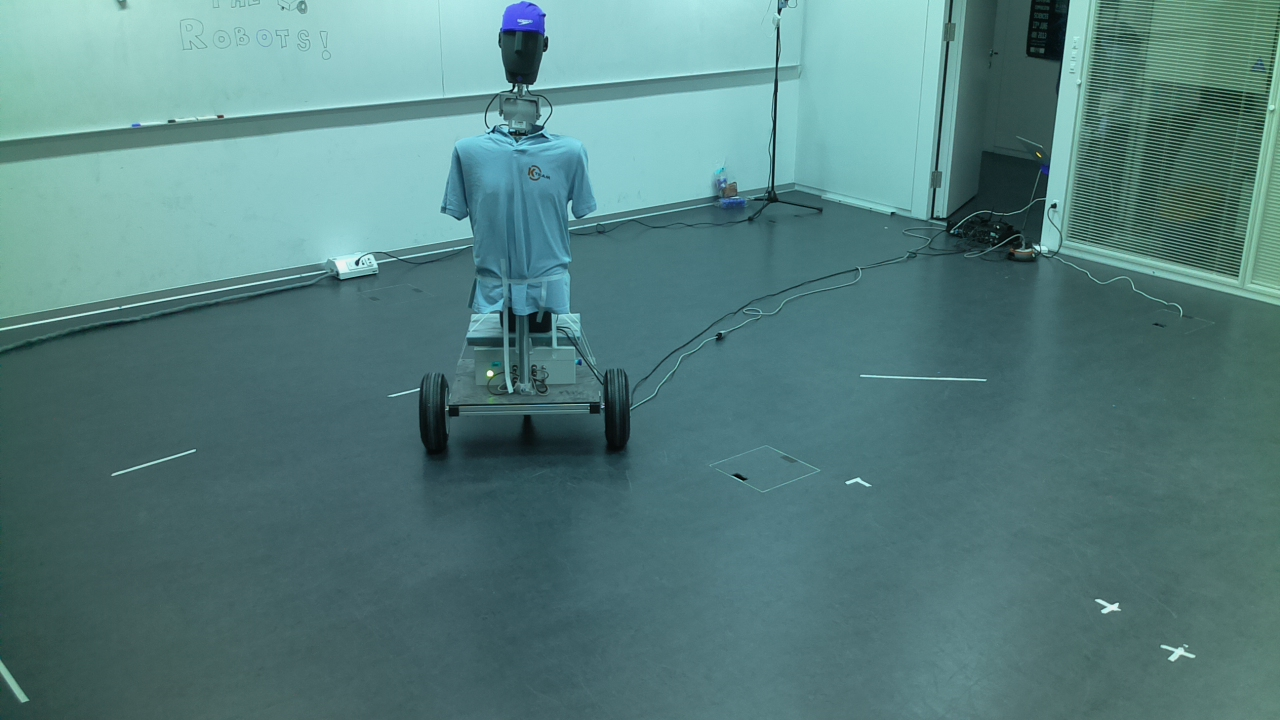
\includegraphics[width=\linewidth]{files/res2_0_image_141.png}
        \caption{View from camera 141 with robot.}
        \label{fig:res2_0_image_141}
    \end{subfigure}
    \begin{subfigure}{0.49\linewidth}
        \centering
        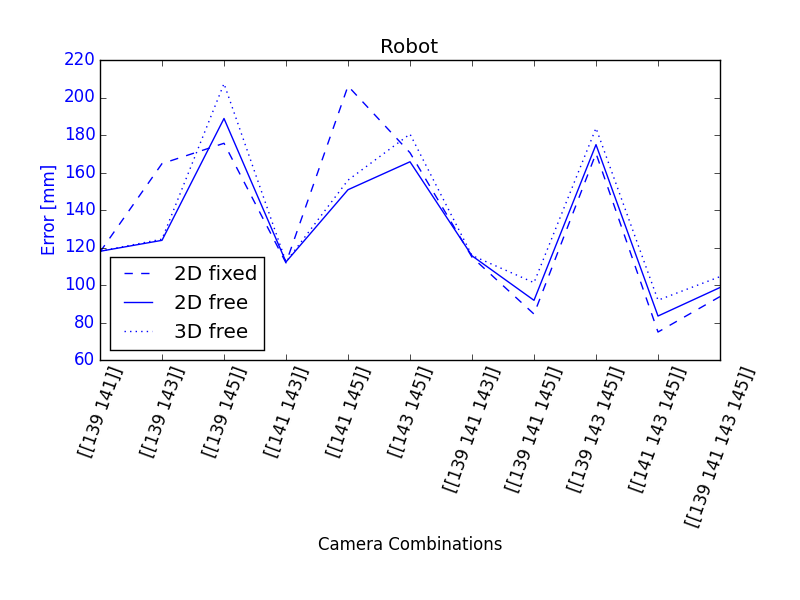
\includegraphics[width=\linewidth]{files/res2_combi_rob.png}
        \caption{2D and 3D errors of robot.}
        \label{fig:res2_combi}
    \end{subfigure}
    \caption{Experiment with checkerboard: view of camera 141 and results of visual localization.}
    \label{fig:experiment2_2}
\end{figure}

In general, the height was very accurately determined to be 1615mm at the first position and 1640mm at the second position (Table \ref{tab:res2_errors}).
The results and the camera positions are shown in Figure \ref{fig:res2_room}.

\begin{table}
\begin{center}
\caption{Experiment with checkerboard: positions obtained with free-height and fixed-height algorithm.}
\begin{tabular}{lcccccc}
\toprule
    & \multicolumn{3}{c}{\textbf{Position 1}} & \multicolumn{3}{c}{\textbf{Position 2}} \\
\midrule
& \textbf{Real} & Free & Fixed & \textbf{Real} & Free & Fixed \\
x   & \textbf{4299} & 4354 & 4331 & \textbf{4014} & 4113 & 4112  \\
y   & \textbf{4304} & 4222 & 4237 & \textbf{4596} & 4579 & 4580 \\
z   & \textbf{1650} & 1615 & 1650 & \textbf{1650} & 1640 & 1650 \\
\bottomrule
\end{tabular}
\label{tab:res2_errors}
\end{center}
\end{table}

\begin{figure}
    \centering
    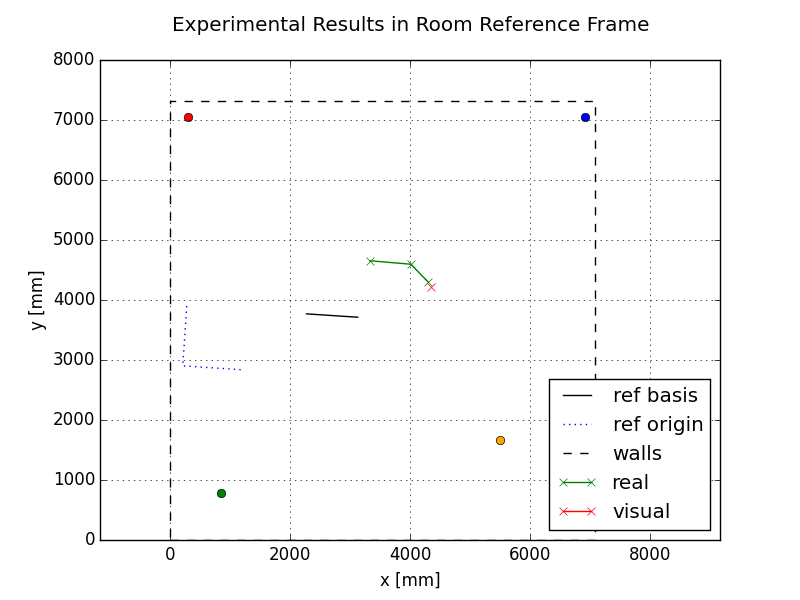
\includegraphics[width=\linewidth]{files/res2_room.png}
    \caption{Experiment with checkerboard: summary of results in room reference frame (Camera numbering: blue 139, red 141, green 143, orange 145).}
    \label{fig:res2_room}
\end{figure}




